\subsection{Background}

\noindent\textbf{Algorithm-Based Fault Tolerance (ABFT).}
ABFT \cite{wang1994algorithm,chen2013online, zhao2020ft} is a method employed to add verifiability of computation on a server by embedding redundancy into data, typically for matrix-based operations. After computation, the resulting redundant result enables the client to verify if the correct result was produced in computation. Due to this property, ABFT enables a system-agnostic error correction directly within the computational algorithms, allowing fault tolerance improvement without relying on external system redundancies or hardware-based solutions. The primary advantage of ABFT is its flexibility. Its flexibility comes from it being hardware-agnostic allowing it to be used in any hardware platform, and from the overheads incurred only when used in computation. 

\begin{figure}[ht]
    \centering
\includegraphics[width=0.9\linewidth]{figures/matrix_checksum.pdf}
    \caption{ABFT in Matrix Multiplication.}
    \label{fig:mat_checksum}
\end{figure}

Figure~\ref{fig:mat_checksum} illustrates the application of ABFT in matrix multiplication. It displays two matrices: matrix \( A \) with an additional checksum row at the bottom and matrix \( B \) on the left. When matrix \( A \) is multiplied by matrix \( A \), the output is matrix \( C \), which also includes a checksum row at the bottom. This checksum row in matrix \( C \) is key to verifying the multiplication process's integrity and correctness. The ABFT approach ensures that any computational errors or discrepancies can be detected through the checksums, thereby providing a reliable method for maintaining the accuracy and integrity of computations in scenarios prone to errors or faults. The inclusion of checksums in matrix operations, as depicted, demonstrates an effective use of redundancy within data structures to enhance computational reliability and security.



% \begin{figure}[htbp]
% \small
%     \centering
%     \[
%     A = \begin{pmatrix}
%         3 & 1 \\
%         1 & 5 \\
%         \textcolor{red}{4} & \textcolor{red}{6} \\
%     \end{pmatrix}
%     \quad
%     \times
%     \quad
%     B = \begin{pmatrix}
%         8 & 3 \\
%         7 & 2 \\
%     \end{pmatrix}
%     \quad
%     =
%     \quad
%     C = \begin{pmatrix}
%         31 & 11 \\
%         43 & 13 \\
%         \textcolor{red}{74} & \textcolor{red}{24} \\
%     \end{pmatrix}
%     \]
%     \caption{An example of matrix multiplication with ABFT checksums. Elements in red are redundant data added for verification.}
%     \label{fig:example_ABFT}
% \end{figure}


\begin{figure}[ht]
    \centering
    \includegraphics[width=0.7\linewidth]{figures/example_ABFT.pdf}
    \caption{An example of matrix multiplication with ABFT checksums. Elements in red are redundant data added for verification.}
    \label{fig:example_ABFT}
\end{figure}


% A simplified example is illustrated in Figure~\ref{fig:example_ABFT}, where a matrix \(A\) is multiplied by matrix \(B\) to produce matrix \(C\). Matrices \(A\) and \(C\) are both initially $2\times 2$. The last row (in red) in matrix \(A\) was added as redundant elements to enable ABFT verification. Each element is calculated as a simple checksum, a summation of original elements in each corresponding column, e.g. $4 = 3+1$. After Matrices \(A\) and \(C\) are multiplied, the resulting matrix \(C\) also contains an additional row. Moreover, under error-free execution, the property that each redundant element in the resulting matrix \(C\) is a simple checksum of each column is retained, e.g. $74 = 31+43$. Therefore, if there is an error affecting memory (e.g. the value of an element in Matrices \(A\), \(B\), or \(C\) is corrupted), or affecting logic (e.g. an error in a functional unit that performs addition or multiplication), the checksums in the resulting matrix will mismatch with the sum of elements in the corresponding column. This simple example illustrates that ABFT technique is capable not only keeping the integrity of data against random errors, but also verify the correctness of matrix multiplication. 

A simplified example is illustrated in Figure~\ref{fig:example_ABFT}. Matrix \(A\) is multiplied by matrix \(B\) to produce matrix \(C\), with both matrices initially \(2\times 2\). An additional row in matrix \(A\) (in red) acts as a checksum, calculated as the sum of elements in each column (e.g., \(4 = 3+1\)). After multiplication, matrix \(C\) also contains an additional row. In an error-free execution, each redundant element in \(C\) is a checksum of its column (e.g., \(74 = 31+43\)). Any error affecting memory or logic will cause a mismatch in these checksums, thus illustrating ABFT's capability to maintain data integrity and verify matrix multiplication correctness.


Note, however, while ABFT can verify computation when dealing with a random fault, its security is not strong. In the example above, if the attacker changes both values of an element and its checksum, the attacker can evade the verification. For example, the attacker may add the same constant to an element of matrix \(A\) and to the checksum, e.g. change $A_{00}$ to 4 and $A_{02}$ to 5. In the resulting matrix \(C\), $C_{00} = 39$ and $C_{02} = 82$, which passes checksum verification and the attack goes undetected. Finally, while ABFT can verify a simple matrix operation (i.e. multiplication), it has not been demonstrated that it can deal with end-to-end DNN inference. 


\noindent\textbf{Fully Homomorphic Encryption (FHE).}
FHE is an encryption method that permits the execution of computations on encrypted data, termed ciphertexts, without the necessity to decrypt them. This capability ensures that sensitive information remains encrypted throughout the computation process,  enhancing data privacy. 

In FHE, a plaintext space is typically structured as a polynomial ring, for instance, \( R = \mathbb{Z}[X]/(X^N + 1) \), where \( N \) is a power of 2. This polynomial ring can encode more than one value at a time by assigning different coefficients of the polynomial to different data values. The concept of slots arises from this encoding: each coefficient in the polynomial represents a separate ``slot,'' allowing multiple values (e.g., elements of a vector) to be encrypted simultaneously within the same ciphertext.

During the encryption process, a vector \( \vec{v} = (v_1, v_2, \ldots, v_k) \) is encoded into a polynomial where each element \( v_i \) is placed into a distinct slot. For example, if \( \vec{v} \) is encoded into the polynomial \( p(x) = v_1 + v_2x + \ldots + v_kx^{k-1} \), the entire vector can be encrypted at once as a single ciphertext. Operations on this ciphertext, such as addition or multiplication, are performed component-wise in a parallel fashion across all slots. This means that a single homomorphic operation on the ciphertext results in the corresponding operation being applied to each element of the vector simultaneously, known as SIMD (Single Instruction, Multiple Data) operations within FHE.

The main FHE primitives are:
\begin{itemize}
    \item \textbf{FHE Encoding}(\( x \)) \( \to p \): Converts a message \( x \) into a polynomial plaintext format \( p \) that can be processed by the FHE system.
    
    \item \textbf{FHE Key Generation}($1^\lambda$) \( \to (sk, pk) \): Generates a set of keys for the FHE scheme. Here, \( \lambda \) is the security parameter that dictates the strength of the keys. This function outputs a secret key \( sk \), and a public key \( pk \).
    
    \item \textbf{FHE Encryption}(p; \( pk \)) \( \to c \): Encrypts the plaintext \( p \) using the public key \( pk \) to produce the ciphertext \( c \).
    
    \item \textbf{FHE Decryption}(c; \( sk \)) \( \to x \): Decrypts the ciphertext \( c \) using the secret key \( sk \) to recover the original message \( x \).
    
    \item \textbf{FHE Addition}(c, \( \hat{c} \)): Performs an addition operation on ciphertexts \( c \) and \( \hat{c} \), which corresponds to the addition of their respective plaintexts. This operation does not require the evaluation key.
    
    \item \textbf{FHE Multiplication}(c, \( \hat{c} \); \( pk \)): Conducts a multiplication operation on ciphertexts \( c \) and \( \hat{c} \), corresponding to the multiplication of their respective plaintexts. This operation typically requires the evaluation key \( pk \) to process the multiplication homomorphically.
\end{itemize}

Non-linear operations are not supported natively in FHE. Hence, a non-linear activation function in a DNN may be approximated by a polynomial function \cite{cryptonet1,cryptonet2, cryptonet3} or a lookup table \cite{lut}.  

\subsection{Related Works} 

Building upon the foundational concepts introduced in the previous subsection, it is essential to also review the performance and overhead considerations before proposing our method in Section~\ref{sec:design}, as high overheads are often impediment to deployment in real systems. Our evaluation of different FHE verification methods is guided by several critical factors that directly influence their practical applicability and effectiveness:

% \begin{itemize}
% \item \textbf{Overheads:} 
% Overheads include space overheads (addition of metadata or magnification of data relative to the original data) and computation overheads (addition of execution time  introduced by the verifiablity). These costs may be incurred both at the server and the client side. It is crucial for a verifiable scheme to keep space and computation overheads low on both ends, especially at the client, where the initial encryption and encoding take place.
% \item \textbf{Scalability:} 
% Ideally, the scheme should scale effectively with the computation size, meaning the overhead relative to the computation size should remain stable or, ideally, diminish. This involves efficient handling of encryption and decryption at the client and managing the computational burden in the server. 
% \item \textbf{Security:} 
% Verifiability should extend beyond just trusted servers; it must also guard against malicious servers with the capability and intent to tamper with data and computations.
% \end{itemize}



\noindent\textbf{Overheads.} 
Overheads include space overheads (addition of metadata or magnification of data relative to the original data) and computation overheads (addition of execution time  introduced by the verifiablity). These costs may be incurred both at the server and the client side. It is crucial for a verifiable scheme to keep space and computation overheads low on both ends, especially at the client, where the initial encryption and encoding take place.

\noindent\textbf{Scalability.} 
Ideally, the scheme should scale effectively with the computation size, meaning the overhead relative to the computation size should remain stable or, ideally, diminish. This involves efficient handling of encryption and decryption at the client and managing the computational burden in the server. 

\noindent\textbf{Security.} 
Verifiability should extend beyond just trusted servers; it must also guard against malicious servers with the capability and intent to tamper with data and computations.

\newcommand*\feature[1]{\ifcase#1 -\or\LEFTcircle\or\CIRCLE\fi}
\newcommand*\f[1]{\feature#1}
\makeatletter
\newcommand*\ex[4]{#1&\f#2&\f#3&\f#4}
\begin{table}[ht]
\centering
\footnotesize
\begin{threeparttable}
\caption{Comparison of current FHE verifiablity schemes and our DataSeal method.}
\label{tab:features}
\setlength{\tabcolsep}{5pt}
\begin{tabular}{lccc}
\toprule
\textbf{Scheme} & \textbf{Scalability} & \textbf{Security} & \textbf{Low Overhead} \\
\midrule
\ex{FHE+ABFT~\cite{Awadallah2021, cryptoeprint:2023/231}}{2}{0}{2}\\
\ex{FHE+MAC~\cite{chatel2022verifiable}}{0}{2}{0}\\
\ex{FHE+ZKP ~\cite{viand2023verifiable}}{0}{2}{0}\\
\ex{FHE+TEE~\cite{natarajan2021chex, viand2023verifiable} }{2}{2}{0}\\
\ex{\textbf{DataSeal}}{2}{2}{2}\\
\bottomrule
\end{tabular}
\begin{tablenotes}
\begin{small}
\vspace{0.1in}
\item $\feature2=\text{provide property}$;
$\text{\feature0}=\text{not provide property}$;
\end{small}
\end{tablenotes}
\end{threeparttable}
\end{table}


In Table \ref{tab:features}, we compare our DataSeal method with existing FHE integrity schemes, highlighting key differences in scalability, security, and overhead. FHE+MAC combines message authentication codes with FHE to ensure data integrity but often suffers from scalability issues and high overhead \cite{chatel2022verifiable}. FHE+ZKP uses zero-knowledge proofs to verify computation correctness without revealing underlying data, providing strong security but also at a significant computational cost \cite{viand2023verifiable}. FHE+TEE leverages Trusted Execution Environments to enhance security, offering better scalability but still limited in reducing computational overhead \cite{natarajan2021chex, viand2023verifiable}. In contrast, as we will demonstrate, our DataSeal approach maintains high scalability and security while significantly minimizing overheads. 

The analysis in Figure~\ref{fig:mot} provides insights into the performance of various Full Homomorphic Encryption (FHE) schemes, focusing on time and memory requirements during client Encoding, server Operation, and client Decoding phases. Unlike ZKP-based schemes, which introduce additional computational steps, the overhead in Message Authentication Code (MAC) based schemes stems from a different process. 



% \begin{figure}[ht]
%     \centering
%     \includegraphics[width=0.47\textwidth]{figures/BGV-TEE.png}
%     \caption{Performance degradation of current state-of-the-art FHE verifiability schemes. (Setup time and Compute time). Refer to Section~\ref{sec:setup} for the platform that was used.}
%     \label{fig:mot}
% \end{figure}

\begin{figure}[ht]
    \centering
    \hspace{-0.5cm}
    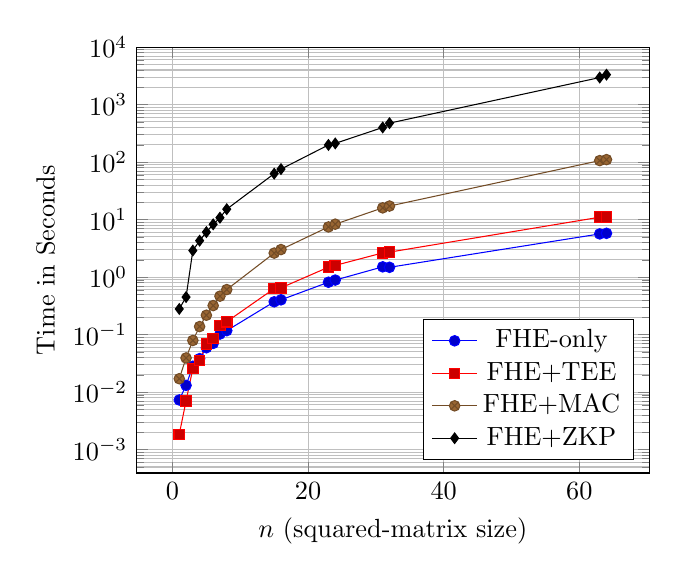
\begin{tikzpicture}[scale=0.95]
\begin{axis}[
    xlabel={$n$ (squared-matrix size)},
    ylabel={Time in Seconds},
    legend pos=south east,
    grid=both,
    ymode=log,
    log basis y={10},
    % xmin=1, xmax=100
    ymax=10000
]
\addplot table {
n   FHE-only
1 0.007317
2 0.013145
3 0.028241
4 0.038275
5 0.059206
6 0.070476
7 0.102446
8 0.117411
15 0.372756
16 0.403254
23 0.815831
24 0.889485
31 1.511596
32 1.483812
63 5.648339
64 5.786344
};
\addlegendentry{FHE-only}

\addplot table {
n   FHE+TEE
% 1 0.2861526045
% 2 0.4250088012
% 3 0.9059316494
% 4 1.245569328
% 5 1.877960703
% 6 2.296731708
% 7 3.317939808
% 8 3.755196614
% 15 11.9755
% 16 12.6607
% 23 25.6463
% 24 27.9983
% 31 48.3255
% 32 47.1153
% 63 177.463
% 64 182.8674
1	0.001850825
2	0.007028951
3	0.02573094
4	0.035254825
5	0.068667673
6	0.086054113
7	0.143496646
8	0.167906306
15	0.632765274
16	0.651516493
23	1.491599519
24	1.600757154
31	2.641528615
32	2.722580376
63	11.02929701
64	11.03712042
};


\addlegendentry{FHE+TEE}

\addplot table {
n   FHE+MAC
1 0.017121
2 0.039324
3 0.079246
4 0.138299
5 0.217848
6 0.320366
7 0.467224
8 0.608021
15 2.62271
16 3.01912
23 7.47015
24 8.3456
31 16.02885
32 17.24404
63 106.3151
64 110.6386
};
\addlegendentry{FHE+MAC}

\addplot[mark=diamond*] table {
n   FHE+ZK
1	0.28
2	0.45
3	2.9
4	4.312174
5	6.077391
6	8.296522
7	10.81826
8	15.20609
15	63.04348
16	75.65217
23	199.2174
24	211.8261
31	400.9565
32	476.6087
63	2958
64	3321.13
};
\addlegendentry{FHE+ZKP}


% \addplot table {
% n   our blind hash
% 1 0.014864
% 2 0.021602
% 3 0.029923
% 4 0.05047
% 5 0.062579
% 6 0.093396
% 7 0.107581
% 8 0.142719
% 15 0.389692
% 16 0.458695
% 23 0.864148
% 24 0.944308
% 31 1.482416
% 32 1.613285
% 63 5.818095
% 64 6.149052

% };
% \addlegendentry{our blind hash}

\end{axis}
\end{tikzpicture}




    \caption{Performance degradation of current state-of-the-art FHE verifiability schemes. (Setup time and Compute time). Refer to Section~\ref{sec:setup} for the platform that was used.}
    \label{fig:mot}
\end{figure}


\noindent\textbf{FHE+ZKP.}
ZKP-based schemes~\cite{ganesh2021rinocchio} are built on ZKP backends such as Pinicchio~\cite{parno2016pinocchio} and Groth16~\cite{groth2016sgroth16}. However, as shown in Figure \ref{fig:mot}, they typically pose heavy computation overheads, primarily resulting from additional calculations at both the client and the server, e.g., the key generation, proof generation, and proof verification. Firstly, the key generation in the setup phase of ZKP-based schemes is typically computationally intensive, which alone can take as many as $30\times$ runtime compared with the FHE-only scheme through all phases. Moreover, the server Operation phase is also hindered by the heavy computation in proof generation, which makes the server operation time $\sim600\times$ longer. Most importantly, the proof verification over ciphertext also introduces heavy overhead to the Client Decoding phase, where the client spends $\sim400 \times$ more time decoding and verifying the proof than FHE-only schemes. 

\noindent\textbf{FHE+MAC.}
The MAC-based approach in homomorphic encryption, exemplified by systems like VERITAS \cite{chatel2022verifiable}, employs Message Authentication Codes (MACs) integrated with ring learning with error schemes to safeguard both the integrity and privacy of data in server computations. In this methodology, each scalar value of an input vector is transformed into an extended vector that not only encapsulates the original data value but also incorporates challenge values derived from a pseudorandom function. Additionally, the data is replicated multiple times within each vector to enhance security against tampering, hence incurring high space overheads. Given that FHE already incurs high space overheads, additional data magnifications makes deployment highly problematic. 

These extended vectors are then concatenated, forming a robust structure that enables the detection of any data alteration during or after processing. This replication also leads to increased computational overhead. Figure~\ref{fig:mot} shows that FHE+MAC incurs more than an order of magnitude over FHE-only.  
%Conversely, DataSeal employs a novel approach using a data duplication method that compresses data through secret weighted vector-matrix multiplication. This boosts scalability and makes DataSeal an apt solution for extensive big data computations, offering significant advantages over traditional MAC schemes by reducing computational demands and improving operational efficiency.



\noindent\textbf{FHE+TEE.}
Recent studies such as \cite{natarajan2021chex, viand2023verifiable} discuss the use of Trusted Execution Environments (TEEs), which offer scalability and strong confidentiality for non-FHE computations but have limitations in integrity protection and performance when applied to FHE. 

However, TEEs cannot be relied upon for full verification. Many TEEs do not even support full integrity protection. For example, AMD SEV~\cite{AMD_SEV} (through its SnP feature) and Intel Scalable SGX~\cite{Intel_SGX} provide isolation of one enclave from others and from the hypervisor by enforcing the ownership of pages. However, memory tampering can occur without having an ownership of a page, and can even occur without using load/store instruction to the target address. For example, in RowHammer attacks, an enclave data may be altered by another party without that party having direct access to data. An earlier version of SGX did support integrity protection via an integrity tree~\cite{intel2021sgx}, but the support was removed in Scalable SGX to avoid overheads that an integrity tree incurs. 

In addition, verifiability goes well beyond integrity protection and supporting it with TEE is challenging. In order for the client to verify computation performed by the server, the client may need an attestation report to ensure the code executed by the server is the correct one. However, that implies that the client needs to trust the enclave in the server to provide the correct expected measurement. Also, TEE model places the trust boundary on the processor. The combination of these factors mean that FHE on TEE require a larger trust base than what traditional FHE computation requires. 

Furthermore, TEE support is not universal and not hardware-agnostic; it is widely applicable on CPUs, but platforms such as NPUs and many GPUs do not support TEEs. A recent NVIDIA GPU (Hopper architecture) supports an enclave model but broadens the trust boundary to the package beyond just the GPU die. 

Finally, TEEs still incur significant performance drawbacks. They provide confidentiality by encrypting data in memory, which is redundant and unnecessary when data is already encrypted with FHE. 

Additionally, as illustrated in Figure~\ref{fig:mot}, running FHE within a TEE, such as AMD SEV which lacks a comprehensive integrity tree, can slow down the process by nearly 2 times. This showcases the practical limitations of TEEs, especially regarding the drastic reduction in performance and the limited scope of verification they provide.

In contrast, by adapting ABFT and securing it, DataSeal offers a more adaptable and efficient solution than TEE. DataSeal provides full verifiability and is hardware-agnostic, hence it can be deployed in any hardware platform. By building on ABFT, DataSeal also does not incur high-performance penalties. However, unlike ABFT, DataSeal utilizes a client-specific secret key, making it secure against data or computation modifications. DataSeal also avoids redundant data encryption that TEE incurs. 



\noindent\textbf{FHE+ABFT.}
The FHE+ABFT (Fully Homomorphic Encryption combined with Algorithm-Based Fault Tolerance) scheme offers an innovative approach to providing integrity protection and verification for encrypted data computations. By embedding error detection and correction directly within the computational algorithms, FHE+ABFT significantly reduces the computational overhead associated with these processes, making the scheme highly scalable and suitable for large-scale applications. However, despite these advantages, FHE+ABFT falls short in security against more sophisticated threats. 

One notable vulnerability is its susceptibility to attacks by adversaries with access to encryption oracles, a common scenario in client-server computations. Such adversaries can exploit this access to manipulate encrypted data and the associated checksums. By replacing the entire dataset and its corresponding checksum with fraudulent versions, an adversary can bypass the integrity checks that FHE+ABFT is supposed to enforce. This ability to tamper with undetected data severely undermines the scheme's security, making it inadequate in environments where robust protection against active threats is required. Therefore, while FHE+ABFT excels in efficiency and scalability, its security vulnerabilities necessitate further enhancements or additional protective measures to safeguard against malicious manipulations.

